\documentclass[11pt,a4paper]{article}

% --- Packages ---
\usepackage[utf8]{inputenc}
\usepackage[T1]{fontenc}
\usepackage{lmodern}
\usepackage[margin=1in]{geometry}
\usepackage{graphicx}
\usepackage{hyperref}
\usepackage{xcolor}
\usepackage{listings}
\usepackage{booktabs}
\usepackage{enumitem}
\usepackage{amsmath}
\usepackage{float}
\usepackage{caption}
\usepackage{subcaption}
\usepackage{tikz}
\usetikzlibrary{shapes,arrows.meta,positioning}

\hypersetup{
    colorlinks=true,
    linkcolor=blue!70!black,
    citecolor=blue!70!black,
    urlcolor=blue!70!black,
}

\lstset{
    basicstyle=\ttfamily\small,
    backgroundcolor=\color{gray!10},
    frame=single,
    breaklines=true,
    keywordstyle=\color{blue!70!black},
    commentstyle=\color{green!50!black},
    stringstyle=\color{red!70!black},
    showstringspaces=false,
    columns=flexible,
}

% --- Title ---
\title{
    \textbf{Layer10 Assignment}
}
\author{Satwik \\ \small Roll No: 24b2498}
\date{\today}

\begin{document}
\maketitle

\begin{abstract}
This report describes a system that transforms scattered corporate email communications into grounded long-term memory. Using the \textbf{Enron Email Dataset} (CMU mirror), we build an end-to-end pipeline that performs structured extraction via a local LLM (Llama~3.1 8B on Ollama), multi-level deduplication with reversible merges, and constructs a queryable memory graph where every claim is traceable to exact source evidence. The system includes a Streamlit-based visualization layer for interactive exploration and a retrieval engine that returns grounded context packs with citations. We also discuss how the approach adapts to Layer10's target environment (email, Slack, Jira/Linear).
\end{abstract}

\tableofcontents
\newpage

% ============================================================
\section{Corpus}
% ============================================================

\subsection{Dataset Choice}
We use the \textbf{Enron Email Dataset}, obtained from the CMU mirror:

\begin{center}
\url{https://www.cs.cmu.edu/~enron/enron_mail_20150507.tar.gz}
\end{center}

The Enron dataset exercises key challenges relevant to Layer10's goals:
\begin{itemize}[nosep]
    \item \textbf{Email threads}: Forwarding, quoting, and reply chains (artifact dedup challenge).
    \item \textbf{Identity resolution}: Same person appears with different email addresses, display names, and aliases.
    \item \textbf{Rich relationships}: Discussions, decisions, escalations, approvals between people, teams, and projects.
    \item \textbf{Temporal dynamics}: Discussions evolve; decisions are made, revised, and superseded.
\end{itemize}

\subsection{Selection and Processing}
We select 7 active Enron employees' mailboxes covering executive decisions, legal discussions, energy trading, government affairs, and logistics:

\begin{center}
\begin{tabular}{ll}
\toprule
\textbf{User} & \textbf{Role / Domain} \\
\midrule
\texttt{kaminski-v} & VP Research --- technical + business \\
\texttt{dasovich-j} & Government Affairs --- policy debates \\
\texttt{mann-k} & Legal --- discussions \& decisions \\
\texttt{shackleton-s} & Trading --- commercial threads \\
\texttt{lay-k} & CEO --- executive decisions \\
\texttt{germany-c} & Trading --- operational discussions \\
\texttt{farmer-d} & Logistics --- scheduling threads \\
\bottomrule
\end{tabular}
\end{center}

Emails are parsed with Python's \texttt{email} module, grouped into conversation threads by normalized subject line, then filtered to threads with 12--15 messages. The final corpus contains \textbf{12 email threads} with 12--15 messages each, producing rich multi-party discussion data.

\subsection{Reproducibility}
\begin{lstlisting}[language=bash]
python fetch_corpus.py
\end{lstlisting}
This downloads the Enron tar.gz ($\sim$1.7~GB, with resume support), extracts the 7 target mailboxes, parses emails, groups into threads, and saves \texttt{data/raw\_corpus.json}.

% ============================================================
\section{Ontology and Schema Design}
% ============================================================

The ontology is defined in \texttt{schema.py} using Pydantic~v2 for strict typed validation and JSON serialization.

\subsection{Entity Types}

\begin{center}
\begin{tabular}{lll}
\toprule
\textbf{Type} & \textbf{Description} & \textbf{Examples} \\
\midrule
\texttt{User} & Email sender/recipient & \textit{vince.kaminski@enron.com} \\
\texttt{Organization} & Company or external entity & \textit{Enron Corp, FERC, PG\&E} \\
\texttt{Topic} & Discussion subject / theme & \textit{California Energy Crisis} \\
\texttt{Project} & Business project or deal & \textit{Project Raptor} \\
\texttt{Decision} & A decision or policy & \textit{Approve the contract} \\
\texttt{Concept} & General concept or term & \textit{Derivatives, Mark-to-market} \\
\texttt{Component} & System, department, or unit & \textit{Trading Desk} \\
\bottomrule
\end{tabular}
\end{center}

\subsection{Relation Types}

\textbf{Core relations}: \texttt{created}, \texttt{reported}, \texttt{fixed}, \texttt{broke}, \texttt{depends\_on}, \texttt{mentions}, \texttt{decided}, \texttt{assigned\_to}, \texttt{labeled}, \texttt{status\_changed}, \texttt{duplicate\_of}, \texttt{related\_to}, \texttt{caused\_by}, \texttt{blocked\_by}, \texttt{implements}, \texttt{reverted}.

\textbf{Email-specific}: \texttt{sent\_to}, \texttt{forwarded\_to}, \texttt{discussed}, \texttt{approved}, \texttt{escalated\_to}.

\subsection{Evidence Model}
Every claim carries a list of \texttt{Evidence} objects:

\begin{center}
\begin{tabular}{ll}
\toprule
\textbf{Field} & \textbf{Description} \\
\midrule
\texttt{source\_id} & Email message-ID or thread + message index \\
\texttt{exact\_quote} & Verbatim excerpt from the email body \\
\texttt{char\_offset\_start} & Character offset start in source text \\
\texttt{char\_offset\_end} & Character offset end \\
\texttt{timestamp} & ISO~8601, when the email was sent \\
\texttt{author} & Email sender \\
\bottomrule
\end{tabular}
\end{center}

\subsection{Temporal Model}
Claims have dual-time tracking:
\begin{itemize}[nosep]
    \item \texttt{valid\_from}: When the fact became true (event time).
    \item \texttt{valid\_until}: When the fact was superseded (validity time).
    \item \texttt{is\_current}: Whether this is the latest known truth.
\end{itemize}

This handles temporal evolution: e.g., a project is ``approved'' at $T_1$, then ``cancelled'' at $T_2$. Both claims exist; the $T_1$ claim has \texttt{valid\_until}~$= T_2$ and \texttt{is\_current}~$=$~\texttt{False}.

% ============================================================
\section{Extraction Pipeline}
% ============================================================

Implemented in \texttt{extraction.py}, using Ollama with Llama~3.1~8B locally.

\subsection{Extraction Flow}

\begin{enumerate}[nosep]
    \item For each email message, construct a structured prompt instructing the LLM to extract entities and claims.
    \item Call Ollama with \texttt{temperature=0.1} for deterministic output.
    \item Parse JSON response with auto-repair (strip markdown fences, regex extraction, LLM self-repair).
    \item Validate against Pydantic schema; skip invalid/low-confidence items.
    \item Checkpoint after each email thread for resumability.
\end{enumerate}

\subsection{Validation and Repair}
\begin{itemize}[nosep]
    \item \texttt{ValidationError} from Pydantic triggers auto-repair prompts.
    \item Invalid entity types fall back to \texttt{Concept}; invalid relation types fall back to \texttt{related\_to}.
    \item Claims without evidence are discarded (quality gate).
    \item Claims below the confidence threshold ($< 0.5$) are discarded.
\end{itemize}

\subsection{Versioning}
Every claim carries an \texttt{extraction\_version} field (currently \texttt{v1}). Changing the prompt or model requires bumping the version. Backfilling is achieved by deleting \texttt{extracted\_raw.json} and re-running extraction; the checkpoint system handles incremental progress.

\subsection{Quality Gates}
\begin{itemize}[nosep]
    \item \textbf{Confidence threshold}: Claims with confidence $< 0.5$ are dropped.
    \item \textbf{Evidence requirement}: Claims without any evidence are dropped.
    \item \textbf{Schema validation}: Invalid JSON is auto-repaired or skipped.
    \item \textbf{Cross-evidence}: During dedup, claims supported by multiple independent emails get boosted confidence.
\end{itemize}

% ============================================================
\section{Deduplication and Canonicalization}
% ============================================================

Implemented in \texttt{deduplication.py}. Three levels of dedup with full reversibility.

\subsection{Artifact Dedup}
Detects near-identical source texts from email quoting patterns:
\begin{itemize}[nosep]
    \item Strip \texttt{>} prefixed quoted lines (multi-level quoting).
    \item Remove \texttt{--- Original Message ---} forwarded blocks.
    \item Remove \texttt{-----Forwarded by...} blocks.
    \item Strip email signature blocks (\texttt{--} marker).
    \item MD5 fingerprint the cleaned text.
    \item Mark duplicates with pointers to originals.
\end{itemize}

\subsection{Entity Canonicalization (Union-Find)}
\textbf{Exact match}: Lowercase + strip whitespace. ``vince kaminski'' and ``Vince Kaminski'' resolve to the same entity.

\textbf{Semantic match}: Embed entity names with \texttt{all-MiniLM-L6-v2} (sentence-transformers). If cosine similarity $> 0.90$, merge into canonical entity. Example: ``Energy Trading Desk'' and ``ENA Trading'' get merged.

\textbf{Implementation}: Union-Find data structure with path compression for efficient grouping. User-type entities are exempt from semantic matching (email addresses are exact identifiers).

\textbf{Result}: Canonical entity gets the shortest name; all original names become aliases stored on the entity.

\subsection{Claim Dedup}
Claims with identical \texttt{(subject\_id, relation, object\_id)} triples are merged:
\begin{itemize}[nosep]
    \item Evidence lists are \textbf{combined} (not replaced) --- the merged claim retains all source pointers.
    \item Highest confidence is kept.
    \item Earliest \texttt{valid\_from} is preserved.
    \item All merge operations are logged in the audit trail.
\end{itemize}

\subsection{Conflict Resolution (Temporal)}
For single-valued relations (\texttt{status\_changed}, \texttt{assigned\_to}, \texttt{labeled}, \texttt{approved}):
\begin{itemize}[nosep]
    \item Claims are sorted chronologically.
    \item Earlier claims get \texttt{valid\_until} set to the newer claim's \texttt{valid\_from} and \texttt{is\_current = False}.
    \item The latest claim is marked \texttt{is\_current = True}.
\end{itemize}

\subsection{Reversibility}
Every merge creates a \texttt{MergeRecord} in the audit log containing:
\begin{itemize}[nosep]
    \item Original entity/claim snapshots (full JSON).
    \item Merge reason and timestamp.
    \item Source and target IDs.
\end{itemize}
An \texttt{undo\_merge()} function restores originals from snapshots, enabling safe rollback.

% ============================================================
\section{Memory Graph Design}
% ============================================================

Implemented in \texttt{graph.py} using NetworkX \texttt{MultiDiGraph}.

\subsection{Architecture}

\begin{figure}[H]
\centering
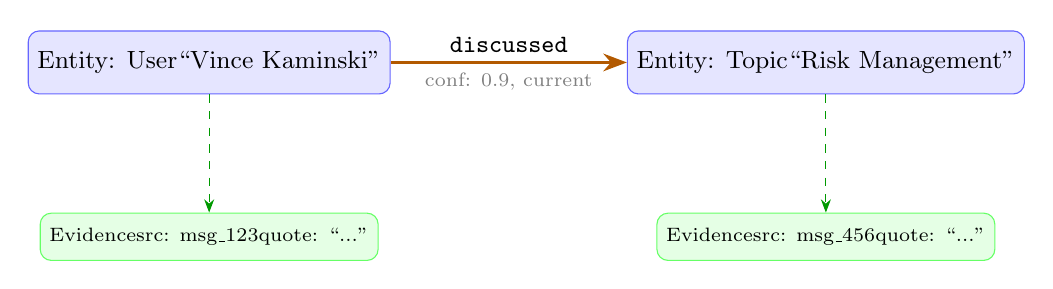
\begin{tikzpicture}[
    node distance=1.8cm,
    entity/.style={rectangle, draw=blue!60, fill=blue!10, rounded corners, minimum width=2.5cm, minimum height=0.8cm, font=\small},
    claim/.style={-{Stealth[length=3mm]}, thick, draw=orange!70!black},
    evidence/.style={rectangle, draw=green!60, fill=green!10, rounded corners, minimum width=2cm, minimum height=0.6cm, font=\scriptsize},
]
    \node[entity] (e1) {Entity: User\\``Vince Kaminski''};
    \node[entity, right=3cm of e1] (e2) {Entity: Topic\\``Risk Management''};
    \node[evidence, below=1.5cm of e1] (ev1) {Evidence\\src: msg\_123\\quote: ``...''};
    \node[evidence, below=1.5cm of e2] (ev2) {Evidence\\src: msg\_456\\quote: ``...''};
    
    \draw[claim] (e1) -- node[above, font=\small] {\texttt{discussed}} node[below, font=\scriptsize, text=gray] {conf: 0.9, current} (e2);
    \draw[-{Stealth}, dashed, draw=green!60!black] (e1) -- (ev1);
    \draw[-{Stealth}, dashed, draw=green!60!black] (e2) -- (ev2);
\end{tikzpicture}
\caption{Memory graph structure: entities as nodes, claims as directed edges, with evidence pointers.}
\end{figure}

\subsection{Core Properties}
\begin{itemize}[nosep]
    \item \textbf{Nodes}: Canonical entities with attributes (name, type, aliases, first\_seen).
    \item \textbf{Edges}: Claims with attributes (relation, evidence list, confidence, temporal validity).
    \item \textbf{Multi-edge}: Multiple directed edges between same nodes (e.g., person \texttt{discussed} and \texttt{approved} same topic).
    \item \textbf{Idempotent}: Entity and claim IDs tracked; re-ingesting the same store is a no-op.
\end{itemize}

\subsection{Time Model}
\begin{itemize}[nosep]
    \item \textbf{Event time}: When an email was sent (\texttt{timestamp} in evidence).
    \item \textbf{Validity time}: When a claim was true (\texttt{valid\_from} / \texttt{valid\_until} on edges).
    \item Queries can filter by \texttt{is\_current} to see only the latest truth, or include historical data.
\end{itemize}

\subsection{Updates and Incremental Ingestion}
\begin{itemize}[nosep]
    \item \textbf{Idempotency}: Entity and claim IDs are tracked; re-ingesting the same store is a no-op.
    \item \textbf{Incremental ingestion}: New email threads can be processed and added without reprocessing existing data.
    \item \textbf{Reprocessing}: Deleting intermediate outputs and re-running the pipeline reprocesses from that stage onward; checkpointing in extraction allows partial re-runs.
    \item \textbf{Edits/deletes}: If a source email is deleted or redacted, claims grounded solely in that source can be flagged as \texttt{redacted} while preserving the claim structure for audit.
\end{itemize}

\subsection{Observability}
\texttt{get\_metrics()} reports:
\begin{itemize}[nosep]
    \item Graph statistics (nodes, edges, connected components).
    \item Entity and relation type distributions.
    \item Evidence quality (avg evidence per claim, claims with no evidence).
    \item Confidence distribution (mean, min, max).
    \item Temporal coverage (current vs.\ historical claims).
    \item Ingestion metrics (duplicates skipped, orphans cleaned).
\end{itemize}

\subsection{Permissions (Conceptual)}
In production, permissions would be enforced at retrieval time:
\begin{itemize}[nosep]
    \item Each evidence pointer includes \texttt{source\_id} traceable to the original email.
    \item A permission layer checks if the querying user has access to the underlying mailbox.
    \item Claims whose evidence is entirely from restricted sources are filtered out.
\end{itemize}

% ============================================================
\section{Retrieval and Grounding}
% ============================================================

Implemented in \texttt{retrieval.py}. Given a natural language question, returns a context pack of ranked, grounded evidence snippets and linked entities/claims.

\subsection{Query Flow}
\begin{enumerate}[nosep]
    \item \textbf{Embed query} using \texttt{all-MiniLM-L6-v2}.
    \item \textbf{Entity matching}: Combine keyword matching (substring search) with semantic similarity against pre-computed entity name embeddings.
    \item \textbf{Graph traversal}: For matched entities, gather all neighboring claims (edges).
    \item \textbf{Ranking}: Score each claim by $\text{entity\_match\_score} \times \text{confidence} \times \text{recency\_boost}$, where recency\_boost $= 1.2$ for current claims and $0.8$ for historical.
    \item \textbf{Context packing}: Top-$K$ claims formatted with full evidence chains.
    \item \textbf{Answer generation} (optional): Send context pack to Ollama with citation instructions.
\end{enumerate}

\subsection{Handling Ambiguity and Conflicts}
\begin{itemize}[nosep]
    \item When multiple entities match, all are included with match scores.
    \item Conflicting claims (historical vs.\ current) are both shown, clearly labeled.
    \item The user can see both sides and click through to evidence in the UI.
\end{itemize}

\subsection{Context Pack Format}
Each context pack contains:
\begin{itemize}[nosep]
    \item \texttt{query}: The original question.
    \item \texttt{matched\_entities}: Entities matched with scores and aliases.
    \item \texttt{items}: Ranked claims, each with subject, relation, object, confidence, temporal status, evidence snippets (source\_id, exact\_quote, author, timestamp), and relevance score.
\end{itemize}

% ============================================================
\section{Visualization Layer}
% ============================================================

Implemented in \texttt{app.py} as a Streamlit web application with 5 interactive pages.

\subsection{Pages}

\begin{enumerate}
    \item \textbf{Graph View}: Interactive pyvis graph with filters (entity type, relation type, confidence threshold, current-only toggle). Nodes colored by entity type; edges show relation labels; hover reveals evidence. Capped at 200 nodes for browser performance.
    
    \item \textbf{Query / Chat}: Text input retrieves a grounded context pack. Shows matched entities, claims with expandable evidence panels, and an optional LLM-generated answer citing sources.
    
    \item \textbf{Evidence Inspector}: Search for any entity to see all connected claims with exact source quotes, authors, and timestamps.
    
    \item \textbf{Merge Inspector}: View entities with aliases (merged), browse the full merge audit log, inspect original snapshots before merge.
    
    \item \textbf{Quality Metrics}: Dashboard showing graph stats, evidence quality, confidence distribution, temporal coverage, entity/relation type distributions.
\end{enumerate}

\subsection{Running the Visualization}
\begin{lstlisting}[language=bash]
streamlit run app.py
\end{lstlisting}

% ============================================================
\section{Layer10 Considerations}
% ============================================================

\subsection{Ontology Adaptation}
\begin{itemize}[nosep]
    \item Add entity types: \texttt{Team}, \texttt{Channel}, \texttt{Thread}, \texttt{Document}, \texttt{Ticket}.
    \item Add relations: \texttt{resolved\_in}, \texttt{referenced\_from}, \texttt{rejected}.
    \item Tickets get structured fields (status, priority, assignee) extracted as typed claims.
\end{itemize}

\subsection{Extraction Contract}
\begin{itemize}[nosep]
    \item \textbf{Slack}: Thread structure gives natural conversation boundaries; reactions and edits tracked as temporal claims.
    \item \textbf{Jira/Linear}: Status transitions are first-class events; custom fields map to the ontology.
    \item \textbf{Cross-system}: Same decision discussed in email + documented in Jira merged with evidence from both.
\end{itemize}

\subsection{Dedup Strategy}
\begin{itemize}[nosep]
    \item \textbf{Unstructured + structured fusion}: Cross-reference Slack discussion threads with Jira tickets via entity canonicalization.
    \item \textbf{Identity resolution}: \texttt{vince.kaminski@enron.com} and \texttt{@vkaminski} on Slack resolve to the same entity.
    \item \textbf{Cross-system dedup}: Same decision discussed across email and Jira merged with evidence from both.
\end{itemize}

\subsection{Grounding and Safety}
\begin{itemize}[nosep]
    \item \textbf{Provenance chains}: Every claim traces back through evidence to original sources.
    \item \textbf{Deletions/redactions}: When a source is deleted, claims grounded in it are marked \texttt{redacted = True} but the claim structure is preserved for audit.
    \item \textbf{Citations}: Generated answers always reference source IDs that can be looked up.
\end{itemize}

\subsection{Long-Term Memory}
\begin{itemize}[nosep]
    \item \textbf{Durable vs.\ ephemeral}: High-confidence claims with multiple independent evidence sources become durable memory; single-evidence, low-confidence claims decay.
    \item \textbf{Drift prevention}: Extraction version tracking; re-extraction with new models creates new version claims for comparison.
    \item \textbf{Incremental updates}: Idempotent ingestion allows processing new emails without reprocessing history.
\end{itemize}

\subsection{Permissions}
Memory retrieval constrained by source access: if a user cannot access the original email thread, claims grounded only in that thread are filtered out. Claims with mixed evidence show only accessible evidence.

\subsection{Operational Reality}
\begin{itemize}[nosep]
    \item \textbf{Scaling}: Graph partitioning by project/team; embedding index uses approximate nearest neighbors (FAISS/Annoy) for large corpora.
    \item \textbf{Cost}: Local Ollama models for extraction (no API costs); embedding model is lightweight ($\sim$80~MB).
    \item \textbf{Evaluation}: Track extraction quality metrics over time; alert on drift (e.g., avg confidence drops).
\end{itemize}

% ============================================================
\section{Architecture and Pipeline Overview}
% ============================================================

\begin{figure}[H]
\centering
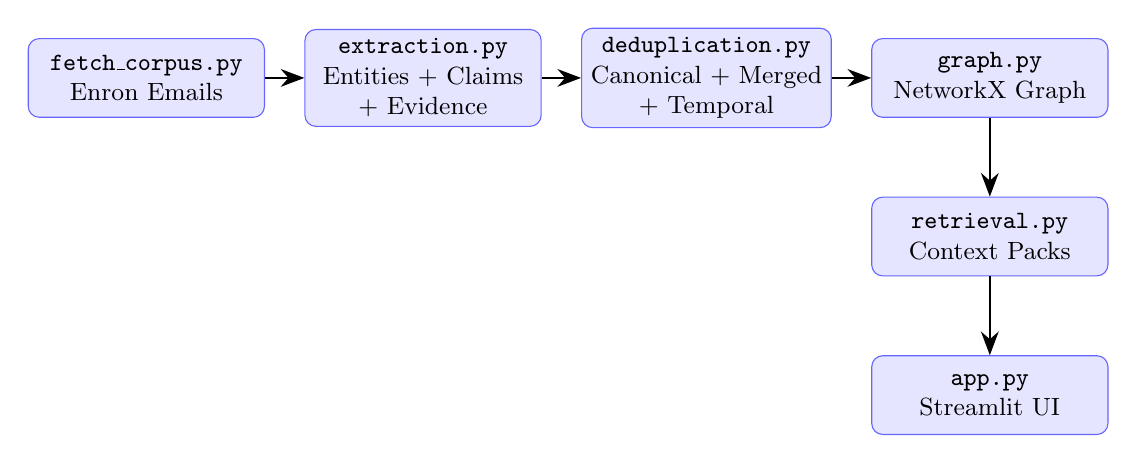
\begin{tikzpicture}[
    node distance=0.5cm,
    block/.style={rectangle, draw=blue!60, fill=blue!10, rounded corners, minimum width=3cm, minimum height=1cm, align=center, font=\small},
    arrow/.style={-{Stealth[length=3mm]}, thick},
]
    \node[block] (fetch) {\texttt{fetch\_corpus.py}\\Enron Emails};
    \node[block, right=of fetch] (extract) {\texttt{extraction.py}\\Entities + Claims\\+ Evidence};
    \node[block, right=of extract] (dedup) {\texttt{deduplication.py}\\Canonical + Merged\\+ Temporal};
    \node[block, right=of dedup] (graph) {\texttt{graph.py}\\NetworkX Graph};
    \node[block, below=1cm of graph] (retrieve) {\texttt{retrieval.py}\\Context Packs};
    \node[block, below=1cm of retrieve] (app) {\texttt{app.py}\\Streamlit UI};
    
    \draw[arrow] (fetch) -- (extract);
    \draw[arrow] (extract) -- (dedup);
    \draw[arrow] (dedup) -- (graph);
    \draw[arrow] (graph) -- (retrieve);
    \draw[arrow] (retrieve) -- (app);
\end{tikzpicture}
\caption{End-to-end pipeline architecture.}
\end{figure}

% ============================================================
\section{Technology Stack}
% ============================================================

\begin{center}
\begin{tabular}{lll}
\toprule
\textbf{Component} & \textbf{Tool} & \textbf{Justification} \\
\midrule
Extraction & Ollama + Llama 3.1 (8B) & Free, local, good at JSON/instruction-following \\
Schema & Pydantic v2 & Strict typed validation, JSON serialization \\
Embeddings & sentence-transformers & Lightweight, local, good semantic similarity \\
Graph & NetworkX MultiDiGraph & In-memory, multi-edge support, Python-native \\
Visualization & Streamlit + pyvis & Interactive web UI, graph rendering \\
Data format & JSON & Human-readable, portable, no DB dependencies \\
\bottomrule
\end{tabular}
\end{center}

% ============================================================
\section{Reproducibility}
% ============================================================

\subsection{Full Pipeline (End-to-End)}
\begin{lstlisting}[language=bash]
# 1. Clone and setup
git clone <repo-url>
cd Layer-10-Assignment
python3 -m venv venv
source venv/bin/activate
pip install -r requirements.txt

# 2. Install Ollama and pull the model
curl -fsSL https://ollama.com/install.sh | sh
ollama serve &          # start Ollama server (if not already running)
ollama pull llama3.1    # download the Llama 3.1 8B model

# 3. Run the full pipeline
python run_pipeline.py

# 4. Launch visualization
streamlit run app.py
\end{lstlisting}

\subsection{Step-by-Step}
\begin{lstlisting}[language=bash]
# Install Ollama (if not already installed)
curl -fsSL https://ollama.com/install.sh | sh
ollama serve &               # start Ollama server
ollama pull llama3.1         # download the model (~4.7 GB)

# Pipeline
python fetch_corpus.py       # Fetch Enron dataset from CMU
python extraction.py         # Extract entities/claims via Ollama
python deduplication.py      # Deduplicate and canonicalize
python graph.py              # Build memory graph
python retrieval.py          # Generate example context packs
streamlit run app.py         # Launch visualization
\end{lstlisting}

\subsection{Output Files}
\begin{center}
\begin{tabular}{ll}
\toprule
\textbf{File} & \textbf{Description} \\
\midrule
\texttt{data/raw\_corpus.json} & Raw corpus (12 email threads) \\
\texttt{data/extracted\_raw.json} & Raw extraction output (entities + claims) \\
\texttt{data/deduped\_store.json} & Deduplicated memory store \\
\texttt{data/memory\_graph.json} & Serialized NetworkX graph \\
\texttt{outputs/deduped\_store.json} & Copy of final store \\
\texttt{outputs/memory\_graph.json} & Copy of final graph \\
\texttt{outputs/example\_context\_packs.json} & Sample retrieval results \\
\bottomrule
\end{tabular}
\end{center}

% ============================================================
\section{Tradeoffs and Design Decisions}
% ============================================================

\begin{enumerate}
    \item \textbf{In-memory graph vs.\ database}: We use NetworkX (in-memory) rather than Neo4j or Postgres for simplicity and zero-dependency setup. For Layer10's production scale, a persistent graph database would be needed.
    
    \item \textbf{Local LLM vs.\ API}: Ollama with Llama~3.1 8B keeps everything free and local. Extraction quality is adequate for the Enron corpus but a larger model (or fine-tuned model) would improve accuracy for complex domains.
    
    \item \textbf{Semantic similarity threshold}: 0.90 for entity merging balances recall (catching genuine aliases) vs.\ precision (avoiding false merges). This was tuned empirically on the Enron data.
    
    \item \textbf{Thread selection}: 12--15 messages per thread balances between having enough context for meaningful extraction and keeping the corpus manageable for local LLM processing.
    
    \item \textbf{JSON storage}: Human-readable and portable, at the cost of query performance at scale. A production system would use a proper database with indexing.
\end{enumerate}

\end{document}
